% File SDSS2020_SampleExtendedAbstract.tex
\documentclass[11pt]{article}
\usepackage{sdss2020} % Uses Times Roman font (either newtx or times package)
\usepackage{url}
\usepackage{latexsym}
\usepackage{amsmath, amsthm, amsfonts}
\usepackage{algorithm, algorithmic}
\usepackage{graphicx}
\usepackage{adjustbox}
\usepackage{setspace}
\setstretch{0.9}
\graphicspath{{images/}}

\title{Artificial Neural Networks and Deep Learning \\
Homework 2}

\author{
  Nicola Dean \\
  10674826 \\
  {\tt nicola.dean \\
  \tt @mail.polimi.it} \\\And
  Marco Fasanella \\
  10617541 \\
  {\tt marco.fasanella \\
  \tt @mail.polimi.it} \\\And
  Raffaello Fornasiere \\
    10790353 \\
    {\tt raffaello.fornasiere \\
    \tt @mail.polimi.it} \\\And
  Christian Spano \\
  10823764 \\
  {\tt christian.spano \\
  \tt @mail.polimi.it} \\}


\date{}

\begin{document}
\maketitle


\section{Introduction}
In this homework, we had to deal with time series. A time series is a sequence of data points that occur in successive order over some period of time. We are given a dataset composed of 2429 sequences each composed of 36 records described by 6 features. In particular, each sequence belongs to a class. Our goal is to build a neural network able to properly classify these data series.\\[0.1cm]
To keep the problem tractable, the chosen learning methods use data from a fixed-length window in the past as an explicit input. The range of possible solutions was limited compared to the previous task; in this case the tests done included Recurrent Neural Networks, ResNet, LSTM, and 1D-CNN models.
\section{Vanilla Models}
We first approached a Vanilla model in order to understand if we could easily tackle the classification problem with a 1D Convolutional Neuronal Network.\\
The best configuration we found consisted in 3 convolutions followed by a Dropout and 2 Dense layers:

This model unfortunately arrived at a result of maximum 0.70 in terms of local Accuracy, reached with a grid search on filters,kernels and dropout.\\
We then moved to a Vanilla LSTM and Bidirectional-LSTM, but with poor results.

\section{Preprocessing}
When it comes to TimeSeries classification/forecasting, preprocessing is a crucial step to grant optimal results.\
In this section will be described all the preprocessing techniques we tried or discarded.
\subsection{Normalization}
After visualizing the data, we noticed that samples has different scale factor based on targets.\
To avoid advantaging some of the classes we decided to normalize the dataset.
\subsubsection{Per Column}
As first approach, we normalized the dataset by \textbf{FULL columns}
\begin{itemize}
  \item \textbf{MinMax} Does not work properly; When applied, the validation accuracy dropped to 33%.
  \item \textbf{Mean / Std} This technique does not improve the accuracy on vanilla models.
\end{itemize}
\subsubsection{Per Sample}
The next method we tried, was to normalize each sample (TimeSeries) independently, to completly remove the different scales of the targets.
\begin{itemize}
  \item \textbf{MinMax} Improve performances but not enough, at least on vanilla models
  \item \textbf{Mean / Std} This was the \textbf{Game Changer} for us, it improves the performances on Vanilla models from 63\% to 67\% on the Vanilla BiLstm
\end{itemize}
\subsection{Augmentation}
In the Homework1 challenge, we noticed the importance of augmentation on this field and so we decided to give it a try also on time series.\
Due to lack of libraries for augmentation of data sequences, we decided to implement our own augmentation techniques.

\subsubsection{Numpy}
Using the function \textit{np.random.normal} it is possible to generate random noise with a certain mean std and shape.\
To obtain augmented samples we copied the dataset multiple time, and then, for each time series, we calculated its standard deviation and applied the augmentation as follow:
\begin{equation*}
    x' = x + w\cdot\mathcal{N}(0, \sigma)
\end{equation*}
where $x$ is a single time series, $x'$ the new (augmented) series, $\sigma$ the standard deviation of $x$ and $w$ an arbitrary weight.

The result of augmentation was immediate and bring us a solid 0.68 using the vanilla BiLstm (that was performing only 0.67 without augmentation)

\subsubsection{More involved augmentation}
In addition to adding noise, we also experimented with various data augmentation techniques including, magnitude warp, time warp, and window slice.
While these techniques led to significant improvements with weaker models, they only resulted in small improvements for more efficient models.
This is likely because more powerful models are already able to effectively extract all the necessary features from the data, so additional augmentation has less impact.
We also tried other methods such as rotation and permutation, but these resulted in a worse overall score.

As part of our experimentation, we tried using autoencoders to denoise the data and generate new samples.
Unfortunately, the results were disappointing.
This was not a surprise, as the effectiveness of an autoencoder is closely tied to the quality of the network used for classification.
In this case, the classification network was not performing well, so it was expected that using it in an autoencoder would also produce suboptimal results.
Despite this, we believe that autoencoders have the potential to be a valuable tool in data preprocessing and will continue to explore their use in future work.

\subsection{Noise Cleaning}
A promising preprocessing technique we guessed was interesting to apply was to get rid of noise, namely, extract just the trend and the seasonal behavior of the time series. Indeed, overall, a time series $x$ can be seen as the sum of three components
\begin{equation*}
    x = trend + seasonal + noise
\end{equation*}
Our goal was to obtain a new data series, $x'$, such that
\begin{equation*}
    x' = trend + seasonal
\end{equation*}
In order to do that, we exploited the \textbf{seasonal\_decompose} function from the \textbf{statsmodels} module. We tried it in different configurations, that is, we tried to place it in different points of the pipeline:
\begin{itemize}
    \item Normalization $\rightarrow$ Augmentation $\rightarrow$ Decomposition
    \item Normalization $\rightarrow$ Decomposition $\rightarrow$ Augmentation
    \item Decomposition $\rightarrow$ Augmentation $\rightarrow$ Normalization
    \item etc...
\end{itemize}
Regardless of the order used, unfortunately, this technique did not give us great results. As a matter of fact, it did not improve the accuracy. Nevertheless, the best configuration was to apply augmentation first and decomposition at the end. The worst configuration, meanwhile, turned out to be the reverse of the just mentioned, that is, decomposition first and augmentation at the end.
\subsection{Expanding Window size}
Another evolution of our preprocessing pipeline was to try combining multiple series of same target (eg: sequences of 2 series concatenated).\
The performance was good but  but since we did not know what data realy are and what was their real meaning we discarded this option almost immediatly.
\subsection{Adding New Features}
In order to further improve the accuracy, we tried to expand the number of features. In particular, what we did was to create new 8 features in which two of them were just the mean and the median of each row, while the remaining ones were computed as follows: for each feature in the original dataset, we generate a new feature just by adding some noise. In other terms, by calling as $x_f$ the time series described by feature $f$, the new time series (feature), $x_f'$, is equal to
\begin{equation*}
    x_f' = x_f + \mathcal{N}(0, \sigma)
\end{equation*}
where $\sigma$ is the standard deviation of $x_f$. Incredibly, this allows us to get up to 0.8250 of accuracy on the test set. However, in Codalab, the performance dropped down dramatically to 0.54. We think that this expansion tries to replicate too much of the dataset we are given and it created some sort of overfitting leading to a poorly generalized model.
\section{Net Concatenations}
Now that our Preprocessing was giving promising results and the possible changes to vanilla models was not giving results better than 0.68
we decided to try combining LSTM and CNN into a single network.
\subsection{CNN + LSTM}
At first we combined an CNN with a LSTM thinking to use the CNN as feature extractor for the LSTM.
This was giving us the same results of BiLstm + Norm + Augm.
\subsection{LSTM + CNN}
We also tried using LSTM to analyze the time series and then CNN as feature extractor for the analyzed data
but the result was the same of BiLstm also in this case.

\section{Inspired By Existing Models}
\begin{figure}[h]
\centering
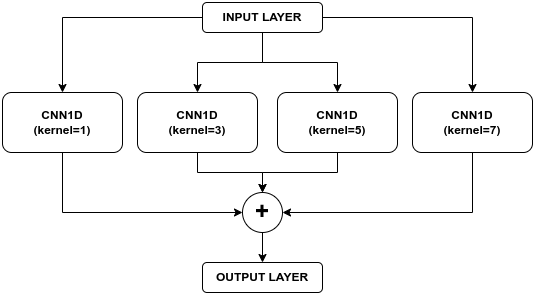
\includegraphics[width=8cm, height=4cm]{Inception}
\caption{CNN1D Inception Like Net}
\end{figure}

\subsubsection{Resnet-CNN1D}
Resnet Model works by adding a big number of layer blocks alternated by some skip layers to avoid vanishing gradient descent.\
We replicated this model in keras using Conv1D instead of the original Conv2D but unfortunatly it has not improved performances and we were still stucked to 68\%.
\subsubsection{Resnet-LSTM}
A second step we had done was to replace the CNN1D with some LSTM like in figure3,
This improved the performances by 0.9\% respect to our best model so far, bringing the accuracy on codalab to 68.9\%.
\begin{figure}[h]
\centering
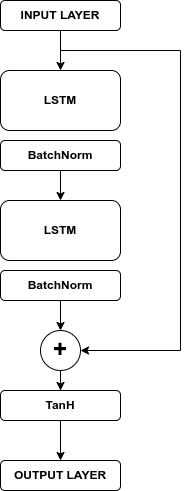
\includegraphics[width=4cm, height=8cm,angle =90]{resnet}
\caption{Resnet Like LSTM Net}
\end{figure}

\section{Heterogeneus Layers}
Not seeing results by contatenating network we thought to create a network of Hybrid layers of LSTM and CNN
\subsection{LSTM + CNN Blocks}
By inspiration on the last laboratories on Time Series forecasting, we tried to create multiple layer of LSTM + CNN
obtaining an improvement in performances from 68\% to 69\% in respect to the vanilla BiLstm.
\subsection{CNN + LSTM Blocks}
We also tried to do the opposite obtaining slightly better results (70\% on submission).
\begin{figure}[h]
  \centering
  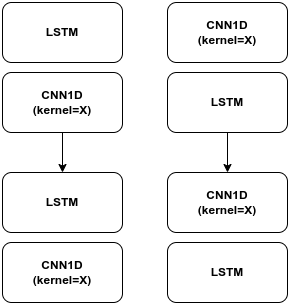
\includegraphics[width=6cm, height=5cm]{LSTMCNN}
  \caption{LSTM-CNN and CNN-LSTM Hybrid Blocks}
\end{figure}

\subsection{CNN + DENSE Blocks}
In an effort to capture more complex relationships between features, we experimented with adding dense layers between an LSTM and CNN network.
Dense layers, also known as fully-connected layers, are a type of neural network layer that allows every neuron in the layer to receive input from all neurons in the previous layer and produce an output for all neurons in the next layer.
This allows dense layers to learn complex relationships between features, which can be especially useful when combined with LSTM and CNN layers which are effective at processing sequential and spatial data, respectively.

However, further attempts to improve performance by modifying the network were made, such as changing the filter size or the number of LSTM units, or adding and removing batch normalization and activation layers, did not result in any additional improvements.
This could be due to the network being unable to learn additional useful patterns from the data, or it could be because the added complexity of the dense layers did not justify the incremental increase in accuracy.
It is important to carefully consider the trade-off between complexity and accuracy when designing a neural network.


\section{Other Models}
In an effort to improve the performance of our classification model, we also tried implementing a 1 vs All approach where we trained one separate model for each class.
Unfortunately, this approach did not work as well as we had hoped, with the network unable to recognize any sequences and classifying them all as "other."
We tried adjusting the ratio of class to other instances in the dataset, as well as building models on top of a pretrained model, but neither of these attempts resulted in significant improvements.

One possible explanation for the poor performance of the 1 vs All approach is that it can be challenging for a neural network to learn to distinguish
classes with very similar features.
Additionally, the network may have struggled to learn useful patterns from the data due to an imbalanced feature distribution or a small dataset size.

After observing that the network was performing poorly on some classes and well on others, we attempted to split the dataset by performance classes in the hope of improving overall score.
The idea is to avoid that the network is biased towards the classes that it performs well on, and instead train it on classes that it struggles to classify.
However, this approach also led to weak results, which could have been due to a lack of data available (and maybe the lack of unique features of some classes) for training.

\section{Our best Model}
Unexpectedly bla bla bla





\section{Conclusion}

\begin{figure}[h]
  \centering
  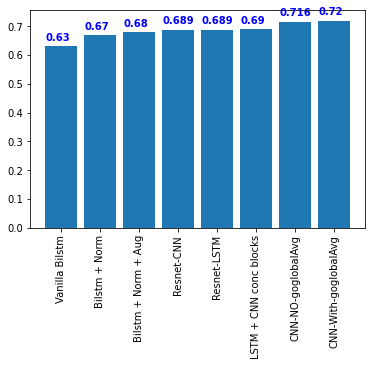
\includegraphics[width=8cm, height=6cm]{chart}
  \caption{LSTM-CNN and CNN-LSTM Hybrid Blocks}
\end{figure}

\bibliographystyle{sdss2020} % Please do not change the bibliography style
\bibliography{SampleReferencesForExtendedAbstract}

\end{document}
